Avant toute explication, voici le schéma muni d’annotations afin d’identifier plus facilement chaque élément matériel.\\

\begin{figure}[H]
    \begin{center}
        \frame{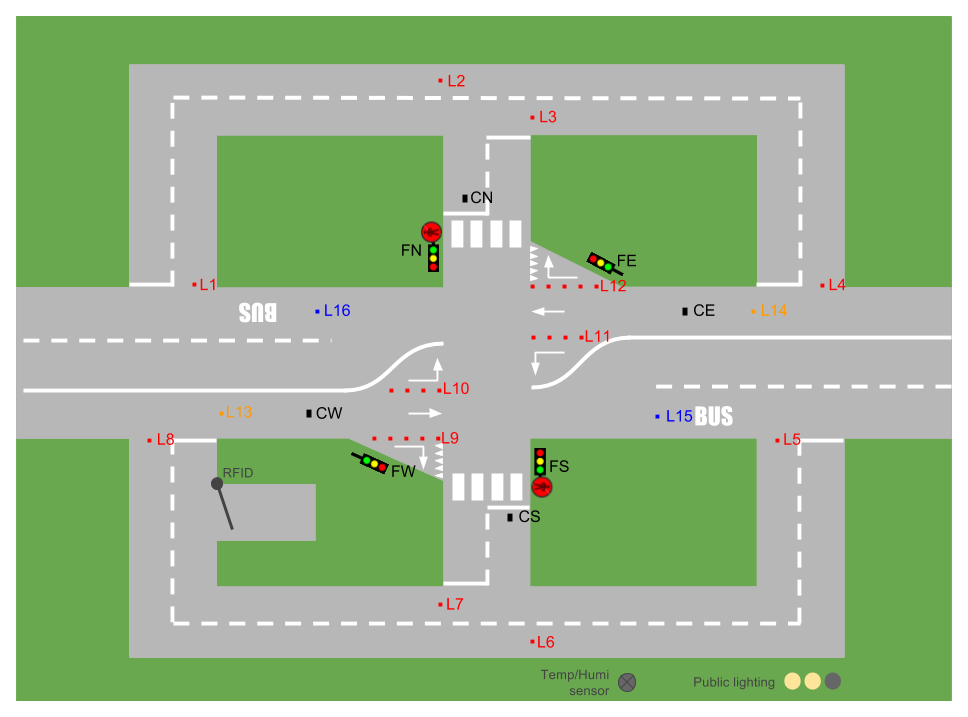
\includegraphics[width=\linewidth, height=\textheight,keepaspectratio]{img/maquette-materiel}}

        \caption{Maquette annotée avec les éléments matériels}
    \end{center}
\end{figure}

La partie hardware sera divisée en deux parties principales. Dans un premier temps, l’Arduino et l’ensemble des capteurs, des LEDs et des affichages lui étant connectés seront abordées. Deuxièmement, l’ensemble des interfaces Phidgets vous seront détaillées, évidemment les précisions les plus précises seront apportées à l’InterfaceKit 8/8/8 qui a recueilli une multitude de capteurs et de LEDs.\\

\subsection{Arduino}
\subsubsection{Élément connectés}
\begin{itemize}
\item \textbf{Les zones piétonnes :}\\
Les LEDs nommées de \textcolor{red}{L1} à \textcolor{red}{L12} permettent la gestion des zones piétonnes. La fermeture d’une zone est symbolisée par l’illumination des LEDs rouges y donnant accès. Si nous souhaitons, par exemple, fermer la zone Nord-Est, les LEDs \textcolor{red}{L3} et \textcolor{red}{L4} devront donc être allumées. Concernant les rangées de LEDs (\textcolor{red}{L9} à \textcolor{red}{L12}), celles-ci permettent de couper l’accès à la zone Nord ou Sud. Ces dernières ne seront donc, par exemple, jamais utilisées lorsque seule la zone Nord-Ouest est fermée.
Comme vous pouvez le remarquer, certaines LEDs ou rangées de LEDs ont exactement le même comportement à quelque moment que ce soit. En effet, reprenons l’exemple de \textcolor{red}{L3} et \textcolor{red}{L4}, ces dernières sont toujours allumées ou éteintes en même temps étant donné qu’elles sont propres à la même zone. Il en va de même pour \textcolor{red}{L1} et \textcolor{red}{L2}, \textcolor{red}{L5} et \textcolor{red}{L6}, \textcolor{red}{L7} et \textcolor{red}{L8}, \textcolor{red}{L9} et \textcolor{red}{L11} ainsi que \textcolor{red}{L10} et \textcolor{red}{L12}. Il va de soi que nous avons regroupé les LEDs ayant le même comportement sur des ports (pins) identiques. Un tableau récapitulatif des pins utilisées sur l’Arduino est disponible dans la section \ref{details-techniques}.

\item \textbf{Les voies prioritaires :}\\
La maquette possède deux voies prioritaires, toutes deux situées sur l’axe principal, elles permettent une sortie rapide de la ville. Ces voies prioritaires peuvent être réservées aux véhicules prioritaires (typiquement les bus) ou partagées entre tous les usagers. Afin de signaler aux utilisateurs que la bande est actuellement réservée aux véhicules prioritaires, les LEDs \textcolor{blue}{L15} et \textcolor{blue}{L16} sont activées. Une fois de plus, ces deux LEDs réagissent exactement de la même façon, elles peuvent donc être connectées sur la même pin.

\item \textbf{Les déviations :}\\
Les deux dernières LEDs connectées à l’Arduino sont les LEDs \textcolor{orange}{L13} et \textcolor{orange}{L14}. Ces LEDs permettent, lorsqu’elles sont allumées, de conseiller l’utilisateur de contourner le carrefour principal car un bouchon y a été détecté. Ces deux LEDs n’ont pas le même fonctionnement étant donné que les bouchons sont détectés par les capteurs de présence CE et CW. Lorsqu’un bouchon est détecté au niveau de CE, seule \textcolor{orange}{L14} doit conseiller les utilisateurs d’utiliser les voies secondaires. Les utilisateurs entrant par l’ouest peuvent pénétrer dans la ville par l’axe principal sans aucune problème.

\item \textbf{Les capteurs :}\\
L’unique capteur que l’Arduino gère est un capteur multifonction. Il permet à la fois de capturer l’humidité et la température ambiante. Sa référence est la suivante : \textsc{Dht11}.

\item \textbf{L’écran LCD :}\\
Le dernier élément connecté à l’Arduino est l’écran LCD qui nous permet d’afficher la température et le taux d’humidité actuel.
\end{itemize}

\subsubsection{Détails techniques}\label{details-techniques}
Voici un tableau récapitulatif reprenant l’ensemble des éléments connectés à l’Arduino. Ce tableau reprend évidemment l’élément, la pin à laquelle il est connecté et l’utilisation qui est faite de cet élément.
\begin{table}[H]
\centering
\captionsetup{width=\textwidth}
{\renewcommand{\arraystretch}{1.5}
    \begin{tabular}{| l | l | l |}
    \hline
    \textbf{Élément} & \textbf{Pin} & \textbf{Utilisation}\\
    \hline
    L1 et L2 & 1 & Zone Nord-Ouest\\
    \hline
    L3 et L4 & 2 & Zone Nord-Est\\
    \hline
    L5 et L6 & 6 & Zone Sud-Est\\
    \hline
    L7 et L8 & 5 & Zone Sud-Ouest\\
    \hline
    L9 et L11 & 4 & Zone Sud\\
    \hline
    L10 et L12 & 3 & Zone Nord\\
    \hline
    L15 et L16 & 7 & Voies prioritaires (Bus)\\
    \hline
    L13 & 0 & Déviation Est\\
    \hline
    L14 & A6 & Déviation Ouest\\
    \hline
    Dht11 & A0 & Température/Humidité\\
    \hline
    Écran LCD & 11 (SDA) & Affichage\\
    & 12 (SCL) & Température/Humidité\\
    \hline
    \end{tabular}}
    \caption{Éléments connectés à l'Arduino}
\end{table}

Concernant les LEDs, nous avons utilisé la loi d’Ohm afin de déterminer la résistance qui nous serait utile afin d’éviter une tension trop importante. La loi d’Ohm est la suivante :
\begin{equation}
   R = \frac{U}{T}
\end{equation}
Grâce à cette formule nous avons pu déduire la résistance idéale. En effet nous avons Uet Ià notre disposition. Ureprésente la différence de potentiel et s’exprime en volt. Elle vaut dans notre cas approximativement trois volts. En effet, l’Arduino propose une alimentation de cinq volts or les LEDs ne supportent qu’en moyenne deux volts. La différence de potentiel est dès lors bien de trois volts. Ireprésente quant à lui l’intensité du courant et s’exprime en ampère. Dans notre cas l’intensité du courant vaut 20 mA soit 0,020 A. Dès lors il est facile de calculer la résistance nécessaire afin de ne pas endommager les LEDs.
\begin{equation}
   R = \frac{U}{T} = \frac{3 \mbox{ V}}{0,02 \mbox{ A}} = 150 \mbox{ \textit{Ohm}}
\end{equation}
N’ayant pas de résistance de 150 \textit{Ohm} à disposition nous avons utilisé des résistances de 220 \textit{Ohm} ce qui n’a posé aucun problème.
Les LEDs ne sont pas directement branchées à l’Arduino mais passent préalablement par une breadboard afin de faciliter l’accès à la terre et de simplifier les connexions.\\

Concernant les capteurs et l’écran LCD, ces éléments requièrent plus de pins pour assurer leur fonctionnement. En effet, le capteur d’humidité nécessite en plus de l’alimentation et de la terre une pin pour transférer les valeurs récoltées. L’écran quant à lui, nécessite deux pins de données. Nous avons donc, pour simplifier les connexions, alimenter la breadboard avec les cinq volts directement fourni par l’Arduino. Il nous a donc suffit de connecter l'alimentation de nos éléments à la breadboard pour les alimenter.


\subsection{Phidgets}
\subsubsection{InterfaceKit 8/8/8}
L’InterfaceKit Phidgets comporte huit connexions pour des capteurs quelconque mais également huit sorties et huit entrées binaires. Nous avons utilisé cinq différents capteurs directement connectés à l’InterfaceKit, quatre d’entre eux nous permettent la détection de présence, il s’agit des capteurs IR-Reflective 10cm (CN et CS) et de photo senseurs (CW et CE) que nous avons nous même adaptés afin de les rendre compatibles avec l’InterfaceKit. En plus de ces quatre capteurs de présence, nous avons également un capteur de luminosité Phidgets.
Voici le tableau récapitulatif des ports utilisés pour ces cinq capteurs.
\begin{table}[H]
\centering
\captionsetup{width=\textwidth}
{\renewcommand{\arraystretch}{1.5}
    \begin{tabular}{| l | l | l |}
    \hline
    \textbf{Capteur} & \textbf{Port} & \textbf{Utilisation}\\
    \hline
    PhotoSensor  & 0 & Présence axe Ouest\\
    \hline
    PhotoSensor  & 1 & Présence axe Est\\
    \hline
    IR-Reflective 10cm & 2 & Présence axe Sud\\
    \hline
    IR-Reflective 10cm & 3 & Présence axe Nord\\
    \hline
    Light Sensor 1000 lux & 4 & Luminosité ambiante\\
    \hline
    \end{tabular}}
    \caption{Éléments connectés à l'InterfaceKit}
\end{table}

Comme mentionné plus haut, nous avons dû adapter les photo senseurs afin de les rendre compatibles avec l’InterfaceKit. Pour cela nous avons utilisé le circuit suivant :
\begin{figure}[H]
    \begin{center}
        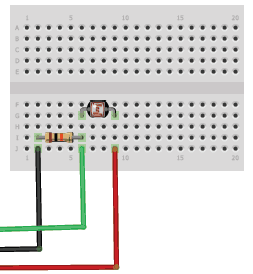
\includegraphics[scale=0.4,keepaspectratio]{img/circuit-photo-senseurs}
    \end{center}
\end{figure}
Le photo senseur est alimenté par l’InterfaceKit (fil rouge), à la sortie du photo sensor, une résistance de 220 \textit{Ohm} est connectée directement à la terre (fil noir) alors que le file vert est branché en série et directement au port de data. Une fois ce montage réalisé, il ne suffit plus que de le connecter à un port de l’InterfaceKit conçu pour les capteurs.\\\\

L’InterfaceKit nous permet également des sorties, nous l’avons donc utilisé pour gérer les feux de signalisation du carrefour principal ainsi que l’éclairage public. FN et FS, en plus des LEDs vertes et rouges pour gérer la circulation, sont munis d’une LED orange afin de signaler aux piétons s’ils peuvent ou non traverser (lorsque la LED est allumée, les piétons peuvent s’engager). Certains feux ont un fonctionnement exactement identique, nous avons donc pu les regrouper sur les mêmes ports de sortie. FN et FS ont le même état quelque soit le moment ainsi que FW et FE.
L’éclairage public est géré par trois LEDs qui peuvent être activées indépendamment en fonction de la luminosité détectée. Lorsque la luminosité ambiante est élevée, aucune LED n’est allumée alors que lorsqu’elle augmente progressivement, les LEDs s’allument les unes après les autres.
Voici le tableau récapitulatif des ports de sorties utilisés pour les feux de signalisation et l’éclairage public :

\begin{table}[H]
\centering
\captionsetup{width=\textwidth}
{\renewcommand{\arraystretch}{1.5}
    \begin{tabular}{| l | l |}
    \hline
    \textbf{Port} & \textbf{Utilisation}\\
    \hline
    0 & Feux rouges FW et FE\\
    \hline
    1 & Feux verts FW et FE\\
    \hline
    2 & Feux rouges FN et FS\\
    \hline
    3 & Feux verts FN et FS\\
    \hline
    4 & Feux piétons FN et FS\\
    \hline
    5 & Eclairage public faible\\
    \hline
    6 & Eclairage public moyen\\
    \hline
    7 & Eclairage public fort\\
    \hline
    \end{tabular}}
    \caption{Ports de sorties utilisés sur l'InterfaceKit}
\end{table}

\subsubsection{Advanced Servo 1-Motor}
Le Phidget Advanced Servo 1-Motor nous permet de gérer la barrière du parking. Le moteur lui est directement connecté et peut être contrôlé via cette interface.

\subsubsection{RFID Read-Write}
Le Phidget RFID Read-Write est lui aussi utilisé pour la gestion du parking et permet l’accès au parking aux utilisateurs enregistrés. Ce dernier est connecté sous la maquette qui, étant en bois, permet la lecture des tags à travers.